%-------------------------------------
% This template comes from Anish Athalye (Unofficial University of Cambridge Poster Template). 

% The Poster Template has been modified by Dr. Rahul Raoniar to fulfill B.Tech/Master/Ph.D./PostDoc student's poster presentation requirements.

% Description: I made this unofficial Poster Template for the Indian Institute of Technology Bombay (IITB). Feel free to use it, modify it, and share it. 

% Thank you note: A huge thanks goes to Anish Athalye for the original template.
%-------------------------------------


\documentclass[final]{beamer}

% ====================
% Packages
% ====================

\usepackage[T1]{fontenc}
\usepackage{lmodern}
\usepackage{amsmath}
\usepackage[orientation=portrait,size=a0,scale=1.0]{beamerposter}
\usetheme{gemini}
\usecolortheme{nott}
\usepackage{graphicx}
\usepackage{booktabs}
\usepackage{tikz}
\usepackage{pgfplots}
\pgfplotsset{compat=1.14}
\usepackage{anyfontsize}
\usepackage{xcolor}
\usepackage[skip=2pt,font=normalsize]{subcaption}
\usepackage{adjustbox}
\usepackage{graphicx}
\usepackage{subcaption}

% ----------------------------------
% For plotting study methodology
% ----------------------------------

\usepackage{tikz}
\usetikzlibrary{shapes.geometric, arrows}

% Defining Tickz Style
\tikzstyle{startstop} = [rectangle, rounded corners, minimum width=3cm, minimum height=1cm, text centered, text width = 10cm, draw=black, fill=white]

% \tikzstyle{io} = [trapezium, trapezium left angle=70, trapezium right angle=110, minimum width=3cm, minimum height=1cm, text centered, text width = 4.5cm, draw=black, fill=blue!30]

\tikzstyle{process} = [rectangle, minimum width=3cm, minimum height=1cm, text centered, text width = 6cm, draw=black, fill=white, text width = 10cm]

% \tikzstyle{decision} = [diamond, minimum width=3cm, minimum height=1cm, text centered, draw=black, fill=green!30]

\tikzstyle{arrow} = [ultra thick,->,>=stealth]


% ====================
% Lengths
% ====================

% If you have N columns, choose \sepwidth and \colwidth such that
% (N+1)*\sepwidth + N*\colwidth = \paperwidth
\newlength{\sepwidth}
\newlength{\colwidth}
\setlength{\sepwidth}{0.025\paperwidth}
\setlength{\colwidth}{0.45\paperwidth}

\newcommand{\separatorcolumn}{\begin{column}{\sepwidth}\end{column}}

% ====================
% Title
% ====================

\title{Exploring Resting-State fMRI-Based Biomarkers for Alzheimer's Disease Detection Using a Functional Data Analysis Approach}

\author{Ido JI \inst{1} \and  Eunjee Lee \inst{2}} 

\institute[shortinst]{
\inst{1} Department of Bio AI Convergence, Chungnam National University
\and
\inst{2} Department of Information and Statistics, Chungnam National University
}

% \samelineand \inst{2} Indian Institute of Technology Guwahati}

% ====================
% Footer (optional)
% ====================

\footercontent{
  \href{}{\textbf{}} \hfill
  \textbf{} \hfill
  \href{mailto:ido.ji@o.cnu.ac.kr}{\textbf{ido.ji@o.cnu.ac.kr}}}
% (can be left out to remove footer)


% ====================
% Logo (optional)
% ====================

% use this to include logos on the left and/or right side of the header:
% \logoright{
\includegraphics[height=6.3cm]{logos/dce_logo.png}}
\logoleft{
\includegraphics[height=8cm]{logos/CNU_logo.png}}

% ====================
% Body
% ====================

\begin{document}

\begin{frame}[t]
\begin{columns}[t]
\separatorcolumn

\begin{column}{\colwidth}

% ----------------------------------
% Research Background
% ----------------------------------
  \begin{block}{Research Background}


\begin{exampleblock}{AD and RS-fMRI}

    \begin{itemize}
      \item \textbf{AD}
      
       Alzheimer's disease (AD) is an incurable brain disorder that slowly destroys memory and thinking skills with brain atrophy.
      
      % \item \textbf{Brain atrophy}
      
      %   Brain atrophy differs between the group with AD and the cognitively normal(CN) group.
      
      % \item \textbf{Neuroimaging method}
      
      %   Neuroimaging techniques are vital in AD research. These methods provide valuable insights into disease progression and contribute to improved diagnostic accuracy and targeted therapeutic interventions.

      \item \textbf{RS-fMRI}

      Resting-state fMRI (rs-fMRI) enables the identification of disrupted functional connectivity patterns and neural network alterations, which can serve as potential biomarkers for early diagnosis and disease progression monitoring.

    \item \textbf{BOLD signal}

    The BOLD (Blood-oxygen-level-dependent) signal of fMRI is an indirect measure of neural activity in the brain.

      
    \end{itemize}

\end{exampleblock}
     
  \end{block}


  






  
%=========================================================
% Section: 연구목적
%==========================================================
\begin{block}{Research Objective}
    \begin{exampleblock}{Functional data analysis (FDA)}

    \begin{itemize}
      \item \textbf{FDA}

        Functional data analysis (FDA) is a statistical approach for analyzing and modeling data that are observed as continuous functions or curves, often collected over time or space.

        \item \textbf{Time-Series Data}
      
        BOLD signal can be regarded as a time series data, so the signal can be treated as a continuous function using FDA. However, this approach have been understudied in AD research.
      
    \end{itemize}

\end{exampleblock}



% \begin{figure}[ht]
%     \centering
%     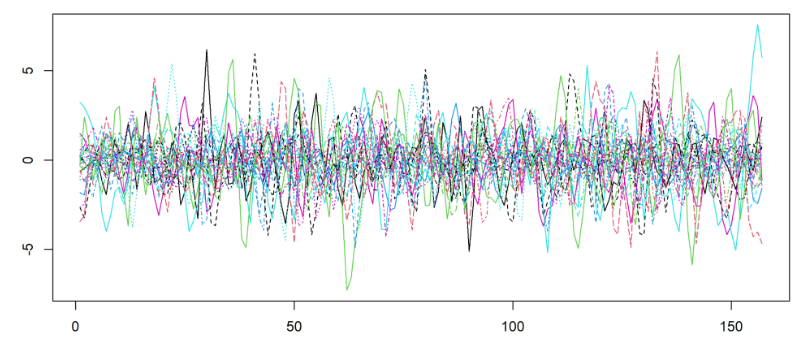
\includegraphics[scale=0.9]{images/Before_expansion.png}
%     \caption{Raw BOLD signals of one ROI}
%     \label{fig:example}
% \end{figure}

    % \heading{asfafasfasf}
    \begin{figure}[ht]
    \centering
    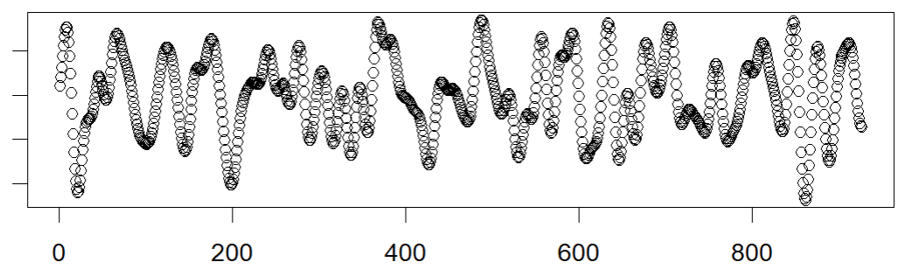
\includegraphics[width=\textwidth]{images/BOLD.png}
    \caption{A BOLD signal observed discretely}
    \label{fig:example}
\end{figure}

  \end{block}


  \begin{alertblock}{objectives}
    \begin{itemize}
      \item \textbf{Objective 1:}

      To identify the brain regions of interest (ROIs) that significantly impact Alzheimer's disease (AD) detection
      
      \item \textbf{Objective 2:} 
      
      To demonstrate that FDA approach leads to improved classification performance when compared to the traditional functional connectivity method
      
    \end{itemize}

  \end{alertblock}





% -------------------------------
% Section: Data collection
% -------------------------------
\begin{block}{Data acquisition}
  \begin{itemize}
    \item The rs-fMRI data was acquired from ADNI(Alzheimer's Disease Neuroimaging Initiative).
    \item The subjects were 24 AD and 221 CN.
    \item For the preprocessing, MATLAB, DPABI, and SPM12 were used.
  \end{itemize} 


    \begin{exampleblock}{Preprocessing pipeline}
        \begin{itemize}
            \item Slice Timing Correction
            \item Head Motion Correction
            \item Nuisance Covariates Regression
            \item Filtering signals
            \item Normalization using EPI template
            \item Extracting BOLD signals from each ROI (Regions of interest)
        \end{itemize}
    \end{exampleblock}


\begin{figure}[ht]
    \centering
    \begin{subfigure}{0.45\textwidth}
        \centering
        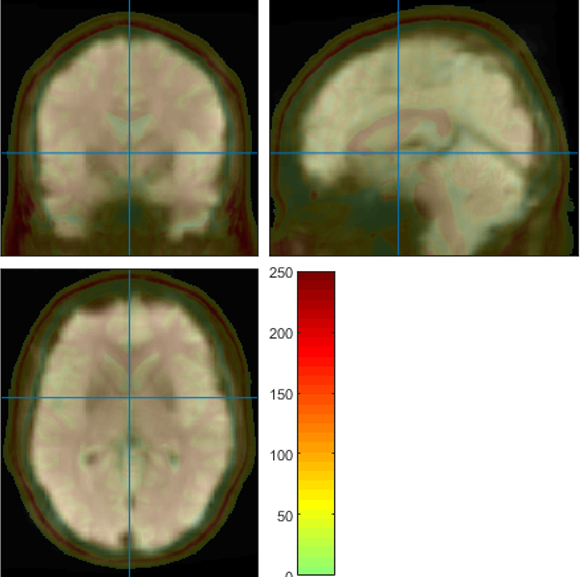
\includegraphics[width=\linewidth]{images/Normalization.png}
        \caption{Normalization of a brain}
        \label{fig:sub1}
    \end{subfigure}%
    \hfill
    \begin{subfigure}{0.45\textwidth}
        \centering
        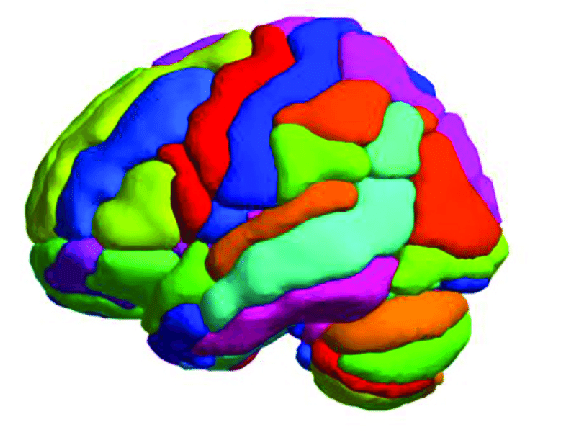
\includegraphics[width=\linewidth]{images/AAL.png}
        \caption{AAL template dividing brain regions into 116 ROIs}
        \label{fig:sub2}
    \end{subfigure}
    \caption{RS-fMRI preprocessing}
    \label{fig:both}
\end{figure}
  
\end{block}











            















\end{column}
\separatorcolumn
\begin{column}{\colwidth}



% -------------------------------
% Section: Descriptive Statistics
% -------------------------------

% \begin{block}{Descriptive statistics}
%     \begin{itemize}
%         \item Sed et augue accumsan nibh 45\% ullamcorper accumsan.
%         \item Sed et augue accumsan nibh ullamcorper accumsan. Nam dictum urna tortor, ut pretium leo eleifend efficitur. 
%         \item Nullam at velit facilisis nibh vulputate porta a sit amet metus.
%         \item Maecenas eget nunc suscipit, luctus nisl non, tristique felis.
%         \item Maecenas tellus diam, placerat sit amet nisl at, dapibus imperdiet arcu.
%     \end{itemize} 
% \end{block}




% ----------------------------------
% Section: Study methodology
% ----------------------------------
 \begin{block}{Classification Modeling}
   \begin{itemize}
            \item  \textbf{B-spline Basis expansion}
            
            B-spline basis expansion is employed to analyze the BOLD signals obtained from resting-state fMRI data for each ROI.
                
        
            \begin{equation*}
                f(t) \approx \sum_{j=1}^{J} c_j \phi_j(t)
            \end{equation*}
    \end{itemize}
\end{block}



            \begin{figure}[ht]
    \centering
    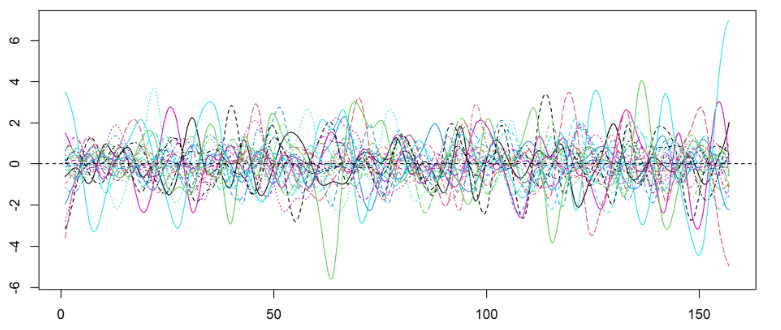
\includegraphics[width=0.7\textwidth]{images/After_expansion.png}
    \caption{BOLD signals smoothed by B-spline basis expansion}
    \label{fig:example}
\end{figure}


\begin{itemize}
    \item \textbf{Functional PCA}

    PC scores explaining more than 90\% for each ROI variation were selected.
\end{itemize}
        
        
     

\begin{itemize}
            \item  \textbf{Group lasso logistic regression} 
            
            The group lasso logistic approach was utilized for both ROI selection and classification tasks using those selected PC scores as features.

            \begin{equation*}
  \hat{\boldsymbol{\beta}} = \arg\min_{\boldsymbol{\beta}} \left\{-\frac{1}{N}\sum_{i=1}^{N} \left[y_i \log(p_i) + (1 - y_i) \log(1 - p_i)\right] + \lambda \sum_{g=1}^{G} w_g \|\boldsymbol{\beta}_g\|_2\right\}
\end{equation*}    
\end{itemize}


 








% -------------------------------
% Section: Results & Discussion
% -------------------------------

\begin{block}{Results and discussion}

\begin{itemize}
    \item \textbf{Model performance}
    
    The classification model demonstrated strong performance, achieving an AUC of 0.9313, which indicates high accuracy in distinguishing between AD and CN.


    \item \textbf{The functional connection}

    The classification model's selected ROIs enable a more focused discussion on the specific brain regions associated with AD research, which are listed in the following table.

    
    
\end{itemize}



\begin{figure}[ht]
    \centering
    \begin{subfigure}{0.4\textwidth}
        \centering
        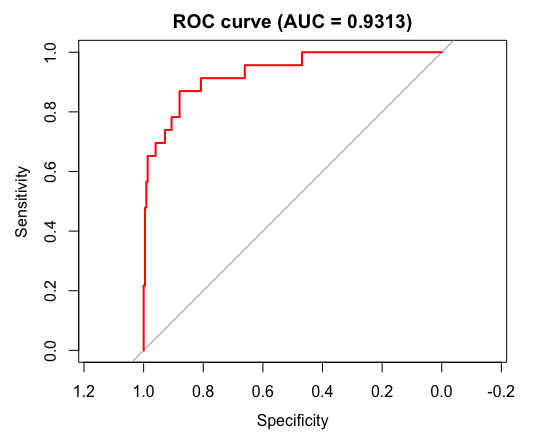
\includegraphics[width=\linewidth]{images/ROC.png}
        \caption{The receiver operating characteristic (ROC) curve and its area under the curve (AUC)}
        \label{fig:sub1}
    \end{subfigure}%
    \hfill
    \begin{subfigure}{0.5\textwidth}
        \centering
        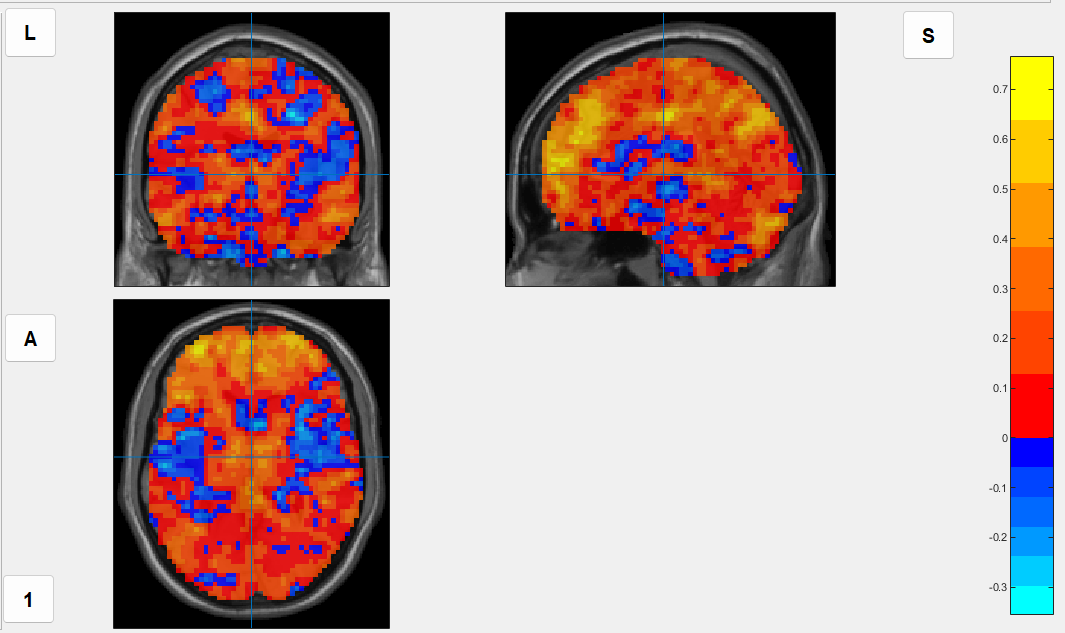
\includegraphics[width=\linewidth]{images/Brain.png}
        \caption{The functional connections map of the shown pairs of ROIs were selected as important factors for the classification}
        \label{fig:sub2}
    \end{subfigure}
    \caption{The results of classification}
    \label{fig:both}
\end{figure}




    
\end{block}








% \begin{table}[]
% \begin{tabular}{|l|l|}
% \hline
% \multicolumn{1}{|c|}{\textbf{ROI}}                                                                                                   & \multicolumn{1}{c|}{\textbf{Functions}}        \\ \hline
% \begin{tabular}[c]{@{}l@{}}right inferior occipital\\ gyrus\end{tabular}                                                             & odor and visual information processing         \\ \hline
% \begin{tabular}[c]{@{}l@{}}dorsolateral area of left superior frontal gyrus\\ left middle frontal gyrus\end{tabular}                 & cognition                                      \\ \hline
% \begin{tabular}[c]{@{}l@{}}orbital part of right middle frontal gyrus\\ \\ orbital part of right inferior frontal gyrus\end{tabular} & processing and responding to external stimuli  \\ \hline
% left precentral gyrusleft rolandic operculum                                                                                         & auditory-motor integration                     \\ \hline
% \begin{tabular}[c]{@{}l@{}}orbital part of left inferior frontal gyrus\\ temporal pole of left superior temporal gyrus\end{tabular}  & stimuli processing from unexpected to expected \\ \hline
% \end{tabular}
% \caption{The representative seleted ROIs and their functions}
% \end{table}






% -------------------------------
% Section: Conclusions
% -------------------------------
   \begin{block}{Conclusions}
    \begin{itemize}
      \item \textbf{Results}
      
      The FDA approach proved effective in AD research, especially classification.

      \item \textbf{Further Study on modeling}
      
      Since there exists a wide array of FDA techniques and group regularization methods, further exploration and application should be needed in future.
      
      \item \textbf{Patients groups}
      Furthermore, exploring preclinical stages between AD and CN groups warrants further investigation.
    \end{itemize}
  \end{block}


% % -------------------------------
% % Section: What is already known about this subject?
% % -------------------------------
%   \begin{exampleblock}{What is already known about this subject?}

%     \begin{itemize}
%       \item \textbf{Lorem ipsum dolor sit amet}, consectetur adipiscing elit. Mauris in nulla ac leo ultricies suscipit.
%       \item The \textbf{Duis vestibulum augue} in leo placerat, sit amet pharetra mi elementum.
%       \item \textbf{Fusce sit amet} velit pulvinar, feugiat velit sit amet, tristique dolor.
%     \end{itemize}

%   \end{exampleblock}

  
% % -------------------------------
% % Section: What does this study add?
% % -------------------------------
%   \begin{exampleblock}{What does this study add?}
%     \begin{itemize}
%       \item Lorem ipsum dolor sit amet, consectetur adipiscing elit. Mauris in nulla ac leo ultricies suscipit.
%       \item The Duis vestibulum augue in leo placerat, sit amet pharetra mi elementum.
%       \item Fusce sit amet velit pulvinar, feugiat velit sit amet, tristique dolor.
%     \end{itemize}

%   \end{exampleblock}


% % -------------------------------
% % Section: Practical Implications
% % -------------------------------
%   \begin{exampleblock}{Practical implications}
%     \begin{itemize}
%       \item Ipsum dolor sit amet, consectetur adipiscing elit. Mauris in nulla ultricies suscipit.
%       \item Duis augue in leo placerat, sit amet pharetra mi elementum.
%       \item Sit amet pulvinar, feugiat velit sit amet, tristique dolor.
%     \end{itemize}

%   \end{exampleblock}

% % -------------------------------
% % Section: References
% % ------------------------------- 

%   \begin{block}{References}

%     \nocite{*}
%     \footnotesize{\bibliographystyle{plain}\bibliography{poster}}

%   \end{block}

% % -------------------------------
% % Section: Portfolio
% % -------------------------------
%   \begin{block}{Author$^{1}$ Portfolio Website}
    
%     \begin{figure}[h]
    \centering
    
\includegraphics[width=0.1\textwidth]{images/portfolio.png}
    \caption*{Scan this QR code}
    \label{fig:figure3}
\end{figure}

%   \end{block}






% -------------------------------
% Section: Acknowledgement
% -------------------------------
\begin{block}{Ackowledgement}
   This material was based on work partially supported by the National Research Foundation of Korea (NRF) grant funded by the Korean government (MSIT) (No. NRF-2022M3J6A1084843, No. NRF-2021R1C1C1013936). This work was also partially supported by the Institute of Information \& communications Technology Planning \& Evaluation (IITP) grant (No.2020-0-01441, No.RS-2022-00155857, Artificial Intelligence Convergence Research Center (Chungnam National University)).
\end{block}














\end{column}
\separatorcolumn



\end{columns}
\end{frame}

\end{document}
